\section{Hardwareentwicklung, Softwarebackend \\ und Benutzeroberfläche \textcolor{gray}{(Simbürger)}}

\subsection{Hardware}



\subsubsection{Planung}
\paragraph{Item}
\paragraph{V-Slot}

\subsubsection{Rahmen}

\subsubsection{X-Achse}

\paragraph{Schlittenauslegung}

\paragraph{Antrieb}

\paragraph{Kabelführung}

\subsubsection{Y-Achse}
\paragraph{Motorauslegung}

\subsubsection{Z-Achse ("Gabel")}
\paragraph{Positionsbestimmung}

Um die optimale Postiton der Zahnriemenaufhängung für die Y-Achse bestimmen zu können, wird überschlagsmäßig ein Massenschwerpunkt in Z-Richtung berechnet.

\noindent\begin{minipage}{\textwidth}
\begin{minipage}[t]{0.5\textwidth}
    \vspace{7mm}
    \begin{equation*}
        X_s = \frac{1}{M} \cdot \displaystyle\sum_{i = 0}^{n} z_i \cdot m_i
    \end{equation*}
\end{minipage}%
\begin{minipage}[t]{0.5\textwidth}
    \begin{align*}
        &Z_s: \text{Z-Koordinate des Massenschwerpunkts} & &\left[m\right]\\
        &M: \text{Gesamtmasse} & &\left[kg\right]\\
        &z_1: \text{Z-Koordinate der Teilmasse} & &\left[m\right] \\
        &m_1: \text{Masse der Teilmasse} & &\left[kg\right]
    \end{align*}
\end{minipage}
\end{minipage} 

\vspace{5mm}


    \begin{table}[h!]
        \centering
        \centering
            \begin{tabular}{c c c}
                Gegenstand & Masse in kg & Position in mm\\
                \hline
                Motor & 0.3 & 21 \\
                Z-Führungsschiene & 1 & 150 \\
                Z-Achse & 0.3 & 180 
            \end{tabular}
        \caption{X-Achse unbeladen und eingefahren}
        \end{table}
        
        \vspace{5mm}
        \begin{table}
            \centering
            \begin{tabular}{c c c}
                Gegenstand & Masse in kg & Position in mm\\ 
                \hline
                Motor & 0.3 & 21 \\
                Z-Führungsschiene & 1 & 150 \\
                Z-Achse & 1.3 & 380
            \end{tabular}
            \caption{X-Achse beim Ladevorgang}
        \end{table}
    
    



\subsubsection{Fertigung}

\subsubsection{Umlenkrollen}
Die Umlenkrollen sind jeweils am Ende der X- und Y-Achsen angebracht. Dadurch dass diese der gesamten Spannkraft ausgesetzt. Dies erfordert spezielle Anforderungen an die Aufhängen als auch an die Umlenkrolle selbst. Diese soll primär eine 180° Wende des Zahnriemens ermöglichen, sowie sekundär eine Führung für den Riemen bieten. 
Umgesetzt wird diese Anforderungen, durch Fertigung von vier Aluminium-Drehteilen in welche Kugellager eingepresst werden.

\begin{figure}[h]
    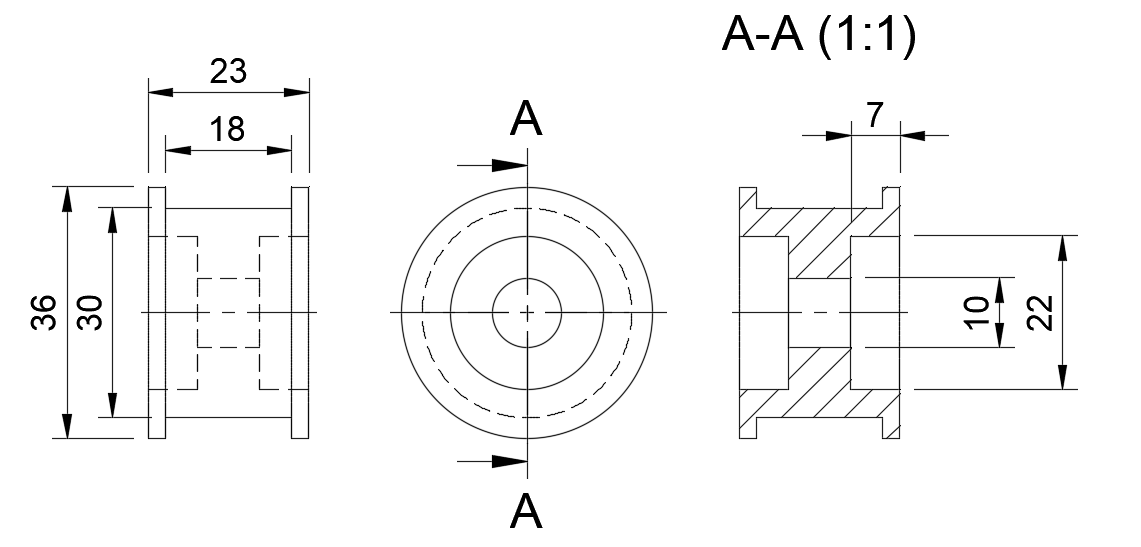
\includegraphics[width=0.5\textwidth]{AT5x16-Umlenkung.png}
    \centering
    \caption{Bauteilzeichnung Umlenkrolle}
\end{figure}

Die Fertigung dieses Teils Lässt sich in folgende Teilschritte unterteilen:
\begin{itemize}
    \setlength\itemsep{0mm}
    \item Zuerst die Frontfläche Plandrehen (900 U/min)
    \item Ungefär 30mm Länge auf das Aussenmaß von 36mm Plandrehen
    \item Mit 9.8mm Bohrer das mittlere Loch vorbohren (540 U/min)
    \item Mit 10mm Reibeisen und viel Öl das Loch auf eine genaue passung bringen (260U/min)
    \item Die Position Relativ zum Backenfutter makieren um beim neu einspannen Rundlaufgenauigkeit gewährzuleisten
    \item Zylinder bei ca. 26 mm Abstechen (540 U/min)
    \item Umspannen und auf maß plandrehen (900 U/min)
    \item Die Aussparung für die Lager mit Eckdrehmeissel beginnen, jedoch nach innen hin nur 6.8 mm 
    \item Bei ca. 17 mm Lochdurchmesser den tatsächleichen Durchmesser mit der Digitalanzeige vergleichen und gegebenennfalls korrigieren
    \item Bei 21.5 mm den Oberschlitten die restlichen 0.2 mm zustellen und die gesamte Tiefe plandrehen
    \item Den Lochdurchmesser auf 21.95 erweitern, und dann in kleinen inkrementen zustellen bis das Lager gerade so nicht passt, um einen Pressitz zu gewährleisten, dies tritt bei Lagern mit 22 mm Aussendurchmesser bei rund 22.04 mm ein.
\end{itemize}

    Durch die Verhältnissmäßig großen Toleranzen bei den Lageraussendurchmessern wird bei 2 der 8 Lagerpassungen zusätztlich Lagerkleber verwendet um eine Zuverlässige Passung zu gewährleisten.

    Da für die Einsparung der Riemenführungsfläche kein Angriffspunkt verfühbar ist wurde auls Halterung ein Dorn gedreht, auf welchen das Drehteil aufgeschraubt wird.

\subsubsection{Lasern}
\subsubsection{Fräsen}


\subsection{Konstruktion}

\subsection{Software und Benutzeroberfläche}

\subsubsection{Grundlegendes}

\subsubsection{Aufbau}

\subsubsection{Benutzeroberfläche}



\subsubsection{Datenbanken}

Als Datenbanksystem wird aufgrund des guten Supports MySQL gewählt. Dies ist ein relationales Datenbankmanagementsystem welches in einem Docker-Container aufgesetzt wird. In diesem werden alle Daten gespeichert, die zur Auswahl sowie zur Ausliferung von Teilen nötig sind.

\begin{figure}[h]
    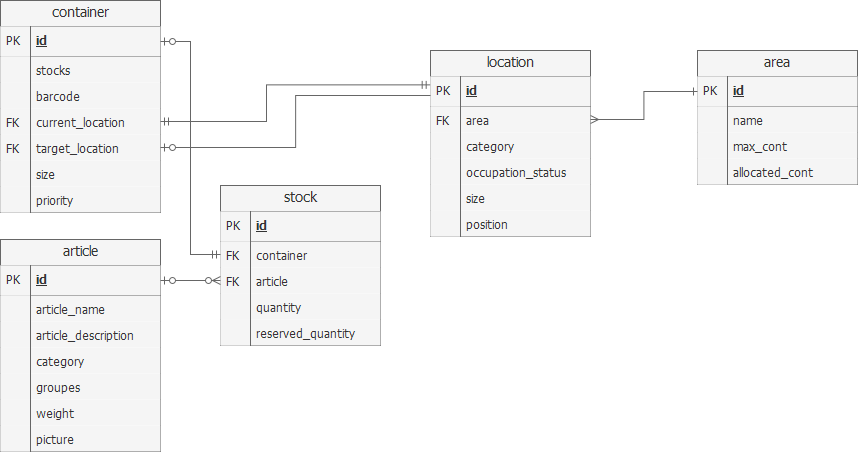
\includegraphics[width=0.6\textwidth]{DB-Schema.png}
    \centering
    \caption{Datenbankschema des AFSS}
\end{figure}

Wie in Abb. 4.2 ersichtlich, beinhäklt sich diese Datenbank fünf Tabellen. Diese hohe Komplexität resultiert daraus, dass diese Struktur eine 100\%ige Flexivilität in der Ablage von Bauteilen in einem überliegendem System bietet.

Die Erste Tabelle beschreibt ein einziges theoretisches Bauteil. Dieses hat einen Namen, Gewicht, Beschreibung und Kategorien zur Filterung. Unter der Spalte 'picture' wird ein Dateiname gespeichert, der zu einem Bild zeigt, dass das Produkt abbildet.
Die zweite beschreibt einen Container. Im Lagersystem entspricht dieser einer Box. Diese kann mehrere `stocks' beinhalten, sowie durch einen Barcode identifiziert werden. Weiters muss jeder Container immer eine aktuelle Position (`current\_location') besitzen, an der die Box gerade ist. Im ausgelagerten (und noch nicht eingelagerten) Zustand ist diese `location' Position 0. Das Ziel der Box wird in `target\_location' gespeichert. Stimmt die aktuelle mit der Zielposition überein, so ist die Box an ihrem Ziel angelangt. Die Kategorie `size' beschreibt die Größe eines Containers und lässt somit theoretisch zu, dass in Zukunft auch unterschiedlich große Boxen zuverlässig in die richtigen Lagerplätze eingelagert werden. `priority' wird nicht verwendet.

Container und Artikel werden im sog. 'stock' verheiratet. Dieser kann als bauteilhaufen in einer Box verstanden werden. Es können also auch mehrere 'stocks' mit dem selben Container geben, dies würde mehreren verschiedenen Bauteilen in einem einzigen Copntainer entsprechen. Auch ist es möglich mehrere Container mit den selben 'stocks' abzubilden, welches ener aufteilung von Abuteilen auf mehrere Container entspräche.

Die Positionen der Container werden in Standorte ('locations') abgebildet. Diese entsprechen den Lagerplätzen. Sie sind einer darüberliegenden 'area' zugeordnet, welche einerseits einen Lagerschrank, aber weiters auch Module wie Vereinzelungsanalgen, abbilden kann. Standorte verfüghen weiters über eine Position welche in X, Y und Z-Richtung beschreibt, wo sich ein Standort im Referenzsystem des Lagers befindet. Auch die größe des Lagerplatzes wird abgebildet, um sicherzustellen, dass auf jeden fall nur die richtige Größe an Box eingelagert wird.


\subsubsection{Docker}

    \begin{wrapfigure}{r}{0.3\textwidth} % 'r' for right, 'l' for left
        \vspace{-20px}
        
\includegraphics[width=0.3\textwidth]{docker-logo-011.png} % Replace with your image file
        \caption{Docker-Logo: \cite{docker_logo}}
    \end{wrapfigure}

    Docker ist eine Umgebung, in der Softwareprojekte isoliert werden können. Da besonders auch bei Projekten mit großem Python anteil, viele Pakete mit verschiedenen Versoinen benötigt werden, ist es sehr hilfreich diese zu bündeln. \\
    Umgesetzt wird dies mithilfe von Containern welche einen gesamten Programmteil als alleinstehende Einheit enthält. Diese werden über ein 'Dockerfile' configuriert, welches sich im selben Ordner wie die Python-Anwendung befindet. In diesem werden Parameter wie die Python-Version und die benötigten pip-Pakete sowie den Programmeinstiegspunkt angegeben. \\ 
    Ein zweier Docker Conteianer wird mit einem MySql-Image erstellt, dort wird die Datenbank aufgesetzt. \\
    Um diese Zwei Container miteinander Kommunizieren zu lasen, ist es ntig ein sog. docker-compose.yml File zu erstellen. Dies enthält alle Informationen über verwendete container, deren Ports, sowie Speicher für Dateien (Volumes). Bei Testbetrieb wird der Datenbankcontainer aleinstehend bestrieben und mit einem anderen Port, keine Zugriffsprobleme zu generieren. In Produktion wird dann derselbe Container in den Containerverband übertragen und dort mit einem anderen Port weiterverwendet. \\
    Erstellt wird dieser Containerverband mit den Consolenbefehlt der auf das docker-compose File zugreift. 
    \begin{lstlisting}[language=bash]
        docker build docker-compose.yml\end{lstlisting}
    Dann werden auch alle Logs in der Kommandozeile ausgegeben sowie 


\subsubsection{Backend}
\subsubsection{APIs}
\subsubsection{Lageralgorithmus}
\subsubsection{Artikelsuche}
\paragraph{TF-IDF und Rust Implementierung} \hspace{0pt} \\
Der TF-IDF (Term Frequency-Inverse Document Frequency) Algorithmus, ist ein Weg um wichtige wörter aus Dokumenten zu extrahieren. Er wird verwendet um beispielsweise in Suchmaschienen, eine Suchanfrage mit Webpagecontent abzugleichen, und die am besten mit der Suchanfrage übereinsteimmenden Dokumente zu sortieren. \\
Im Fall dieser Anwendung werden die Daten aus der Artikeldatenbank als 'Dokumente'  angesehen und die Suchanfrage aus dem Suchfeld wird dafür verwendet um die am besten passenden Artikel zu finden.
\\
Durch den Relativ hohen Rechenaufwand bei dieser Suchoperation wird dieser in der Programmiersprache Rust implementert. Die Implementierung in Rust ist im vergleich zu Python schon bei relativ kleinen Datenmenge bis zu 5-mal schneller.

\subparagraph{Rust}
Rust ist eine sehr effiziente und schnelle Programmiersprache die in den späten 2000er und frühen 2010ern bei Mozilla und der Open-Source-Community entwickelt. Sie unterstützt unter anderem mehr Typensicherheit und verhindert viele Programmierfehler. 

Die Funktion dieses Algorithmus ist in drei unterteile Unterteilt.

\begin{enumerate}
    \item Term Frequenz \\
    Die Termfrequenz gibt an, wie oft ein angegebenes Wort in einem Dokument vorhanen ist. Dies wird durch die Folgende Funktion kalkuliert.
    
    \begin{lstlisting}[language=Rust]
fn term_frequency(document: &str, term: &str) -> f64 {
    // Store the lowercase document as a String to ensure it lives long enough
    let lower_document = document.to_lowercase(); 

    // Split the document into words
    let normalize_document: Vec<&str> = lower_document.split_whitespace().collect();
    // Make sure the searchterm is lowercase
    let normalize_term = term.to_lowercase();

    // Count occurrences of the term in the document
    let count = normalize_document
        .iter()
        .filter(|&&word| word == normalize_term) // Compare each word with the term
        .count();

    // Calculate the term frequency as occurrences / total number of words
    let total_words = normalize_document.len();
    if total_words == 0 {
        0.0 // Avoid division by zero if the document is empty
    } else {
        count as f64 / total_words as f64
    }
}\end{lstlisting}

    Mithilfe dieser wird eine Liste aller Wörter und der Vorkommenshäufigkeit dieser erstellt.

    \item Die zweite Komponente ist dann die Inverse Dokument Frequenz. Diese gewichtet, die Anzahl der Dokumente in dem das gesuchte Wort enthalten ist relativ zur Gesamtdokumentanzahl vorkommt. Häufig vorkommende Worte wie z.B. 'und' werden hierbei weniger gewichtet als einzigartige Wörter.

\begin{lstlisting}[language=Rust]
fn inverse_document_frequency(term: &str, all_documents: &Vec<String>) -> f64 {
    let mut num_documents_with_this_term = 0;

    // Iterate over all documents to check if they contain the term
    for doc in all_documents {
        // Normalize both term and document by converting them to lowercase
        let lower_doc = doc.to_lowercase();
        let normalized_doc: Vec<&str> = lower_doc.split_whitespace().collect();

        // Check if the term exists in the document
        if normalized_doc.contains(&term.to_lowercase().as_str()) {
            num_documents_with_this_term += 1;
        }
    }

    // Calculate IDF
    if num_documents_with_this_term > 0 {
        // Apply the IDF formula: 1 + log(total_documents / documents_with_term)
        1.0 + ((all_documents.len() as f64) / (num_documents_with_this_term as f64)).ln()
    } else {
        // If the term is not found in any document, return 1.0
        1.0
    }
}
\end{lstlisting}

    \item Nun liegt Liste davon vor, wie oft ein Wort in den Suchdaten vorkommt, als auch, wie oft ein Suchbegriff in einem bestimmten Dokument ist. \\ Als nächsten Schritt werden diese beiden Werte für jeden Suchbegriff miteinander multipliziert und ergeben somit einen Vektor der die Suchwörter in Relation zu jedem einzelnen Dokument stellt.
    \item Als letzten Schritt wird der zuvor errechnete Dokumentenvektor (der IDF jedes Suchterms in jedem Dokument) mit dem Suchvektor verglichen. Die geschieht mit der sog. Kosinus-Ähnlichkeit.
    \begin{lstlisting}[language=Rust]
fn cos_similarity(query_p: Vec<f64>, document_p: Vec<f64>) -> f64 {
    // Ensure that both vectors have the same length
    if query_p.len() != document_p.len() {
        return -1.0;
    }

    let mut dot_product = 0.0;
    let mut abs_doc_squared = 0.0;
    let mut abs_query_squared = 0.0;

    // Calculate the dot product and the magnitudes (squared)
    for i in 0..query_p.len() {
        dot_product += query_p[i] * document_p[i];
        abs_doc_squared += document_p[i].powi(2); // document_p[x] ** 2
        abs_query_squared += query_p[i].powi(2); // query_p[x] ** 2
    }

    // Calculate the magnitudes
    let abs_doc = abs_doc_squared.sqrt();
    let abs_query = abs_query_squared.sqrt();

    // Handle division by zero in case of zero vectors
    if abs_doc == 0.0 || abs_query == 0.0 {
        return 0.0;
    }

    // Return the cosine similarity
    return dot_product / (abs_doc * abs_query);
}\end{lstlisting}
    Nach der Berechnung dieser für jedes Dokument werden alle Dokumente sortiert und ausgegeben.
\end{enumerate}






